%\begin{frame}{Test bench}
%	\only<1>{El sistema fue simulado con el objetivo de corroborar el correcto funcionamiento del sistema, cómo así también detectar fallas en la descripción realizada y obtener una forma de depuración de lo realizado.}
%\end{frame}
\begin{frame}{Sistema de pruebas}
	\framesubtitle{Arquitectura}
	\centering
	\begin{tikzpicture}[scale=.53]
		\begin{scope}[transform shape,node distance=4,>=latex,double distance=1.3]
			\node[simple](mea)[]{Máquina de Estados Finitos};
			
			\node[simple,rounded corners](fx2lp)[left=of mea]{Interfaz EZ-USB FX2LP};
			\draw[<->,double]([yshift=10*220/11]fx2lp.south east) --node[above]{FD[15:0]}([yshift=220/11*10]mea.south west);
			\draw[<-,double]([yshift=220/11*9]fx2lp.south east) --node[above]{FADDR[1:0]}([yshift=220/11*9]mea.south west);
			\draw[->]([yshift=220/11*8]fx2lp.south east) --node[above]{FLAGA}([yshift=220/11*8]mea.south west);
			\draw[->]([yshift=220/11*7]fx2lp.south east) --node[above]{FLAGB}([yshift=220/11*7]mea.south west);
			\draw[->]([yshift=220/11*6]fx2lp.south east) --node[above]{FLAGC}([yshift=220/11*6]mea.south west);
			\draw[->]([yshift=220/11*5]fx2lp.south east) --node[above]{FLAGD}([yshift=220/11*5]mea.south west);
			\draw[->]([yshift=220/11*4]fx2lp.south east) --node[above]{SLWR}([yshift=220/11*4]mea.south west);
			\draw[->]([yshift=220/11*3]fx2lp.south east) --node[above]{SLRD}([yshift=220/11*3]mea.south west);
			\draw[->]([yshift=220/11*2]fx2lp.south east) --node[above]{SLOE}([yshift=220/11*2]mea.south west);
			\draw[->]([yshift=220/11*1]fx2lp.south east) --node[above]{PKTEND}([yshift=220/11*1]mea.south west);
			
			
			\node[simple,minimum height=150,minimum width=50](interno)[right=6 of mea.north east,anchor=north west]{Memoria FIFO};
			\draw[double,->]([yshift=-1*150/8]mea.north east)--node[above]{Dato\_enviado[15:0]} ([yshift=-1*150/8]interno.north west);
			\draw[double,<-]([yshift=-2*150/8]mea.north east)--node[above]{Dato\_a\_enviar[15:0]}([yshift=-2*150/8]interno.north west);
			\draw[<-]([yshift=-3*150/8]mea.north east)--node[above]{Enviar\_datos}([yshift=-3*150/8]interno.north west);
			\draw[<-]([yshift=-4*150/8]mea.north east)--node[above]{PKTEND}([yshift=-4*150/8]interno.north west);
			
			\node[simple,minimum height=70](adapt)[anchor=south] at  ($(mea.south|-interno.south)!0.5!(interno.south)$|-interno.south) {Adaptador};
			\draw[->]([yshift=-5.5*150/6]mea.north east)--node[above]{SLWR}([yshift=-5.5*150/6]mea.north east -| adapt.west);
			\draw[->]([yshift=-4.5*150/6]mea.north east)--node[above]{SLRD}([yshift=-4.5*150/6]mea.north east -| adapt.west);
			\draw[<-]([yshift=1*70/5]adapt.south east) --node[above]{Llena} ([yshift=1*70/5]adapt.south east -| interno.west);
			\draw[<-]([yshift=2*70/5]adapt.south east) --node[above]{Vacia} ([yshift=2*70/5]adapt.south east -| interno.west);
			\draw[->]([yshift=3*70/5]adapt.south east) --node[above]{wr\_en} ([yshift=3*70/5]adapt.south east -|interno.west);
			\draw[->]([yshift=4*70/5]adapt.south east) --node[above]{rd\_en} ([yshift=4*70/5]adapt.south east -|interno.west);
			
			\node[simple,minimum size=50](clk) [anchor=south]at (mea.south west-|interno.south)  {PLL};
			\draw[<-]([yshift=15]mea.east |- clk.west)--node[above,near end]{Reloj}([yshift=15]clk.west);
			\draw[->] (clk) -- node[right]{clk} (interno);
			\draw[->] ([yshift=15]clk.west) -| (adapt);
			
			\node[rounded corners,simple, minimum size=50](clkSrc)[right=1 of clk]{Fuente de reloj};
			\draw[->](clkSrc) to (clk);
			
			\node[simple,minimum size=30](rst)[anchor=south]at($(mea.south)!.5!(clk.south)$) {Reset};
			\draw[->]([yshift=15]clk.west)-|(rst.north);
			\node[simple,rounded corners,minimum size=50](puls)[below=1 of rst]{Pulsador};
			\draw[->](rst.west) --node[above]{Reset} (rst.west -| mea.east);
			\draw[<-](rst.south)--(puls.north);
			
		\end{scope}
		\begin{scope}[]
			\node[rounded corners,inner ysep=5pt,draw=blue,dashed,rectangle,fit={(clk)(mea)(interno)},label=north:\scriptsize{FPGA}](fpga){};
			\node[inner ysep=11pt, yshift= 8pt, draw=blue,dash dot,rectangle,fit={(puls)(fpga)(clkSrc)},label=north:\scriptsize{Mojo}](){};
		\end{scope}
	\end{tikzpicture}
\end{frame}

\begin{frame}{Sistema de Pruebas}
	\framesubtitle{Implementación en VHDL}
	\centering
	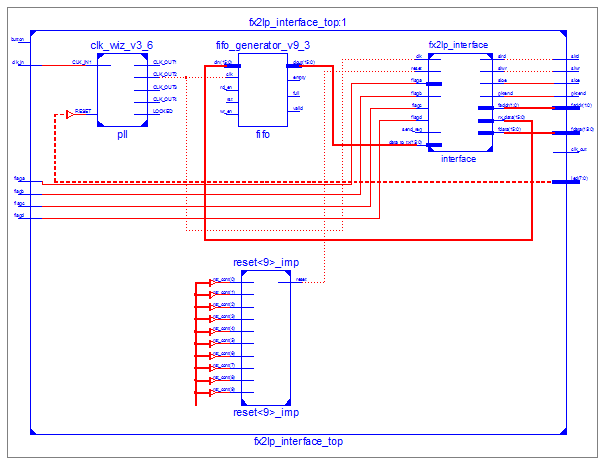
\includegraphics[height=.83\textheight]{fx2lp_rtl}
\end{frame}

\begin{frame}{Verificación Funcional}
	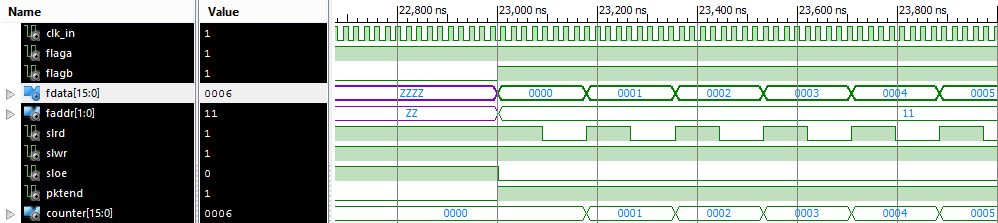
\includegraphics[width=\textwidth]{sist_tb_lect}
\end{frame}

\begin{frame}{Verificación Funcional}
	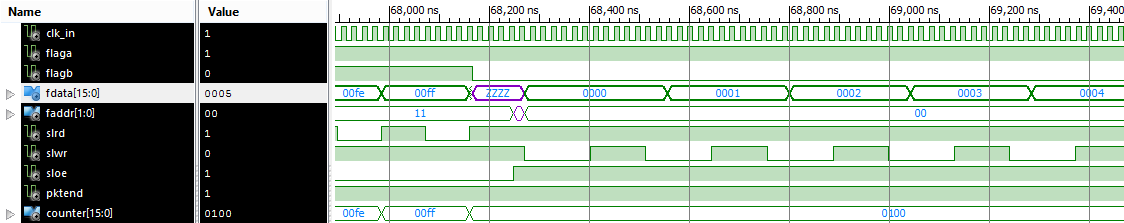
\includegraphics[width=\textwidth]{sist_tb_esc}\\
	\vfill
	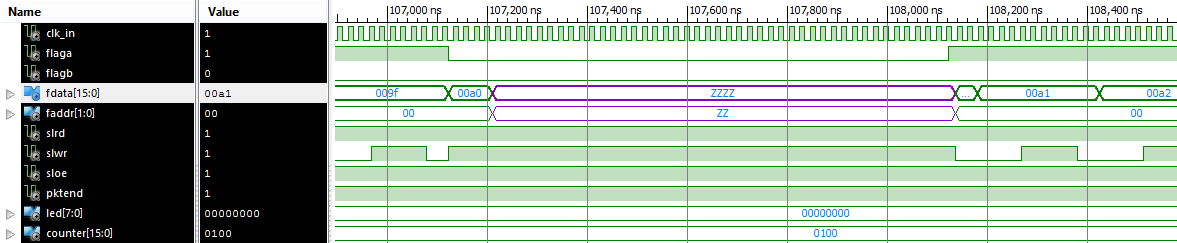
\includegraphics[width=\textwidth]{sist_tb_esc_int}
\end{frame}

\begin{frame}{Verificación Funcional}
	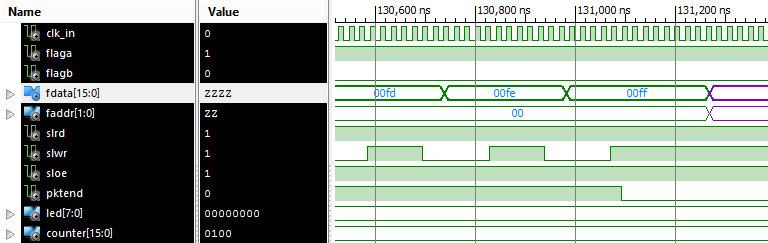
\includegraphics[width=\textwidth]{sist_tb_pktend}
\end{frame}
%\begin{frame}{Test bench - Lectura de la interfaz}
%	\only<1>{
%		\centering
%		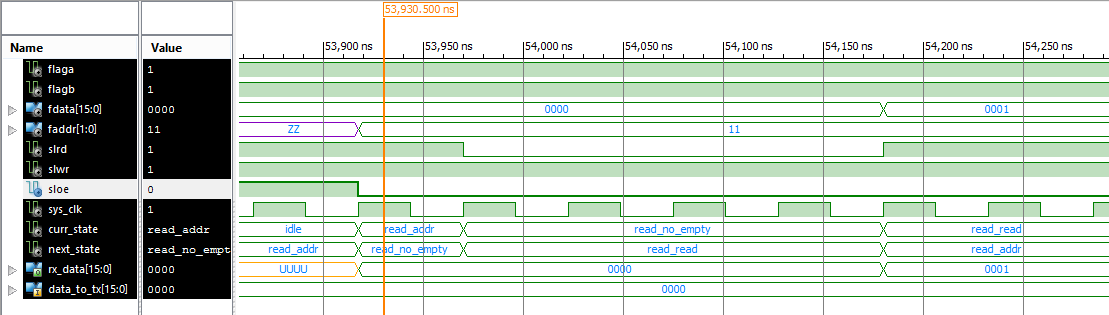
\includegraphics[width=\textwidth]{tb_if_rd_mef}\\
%		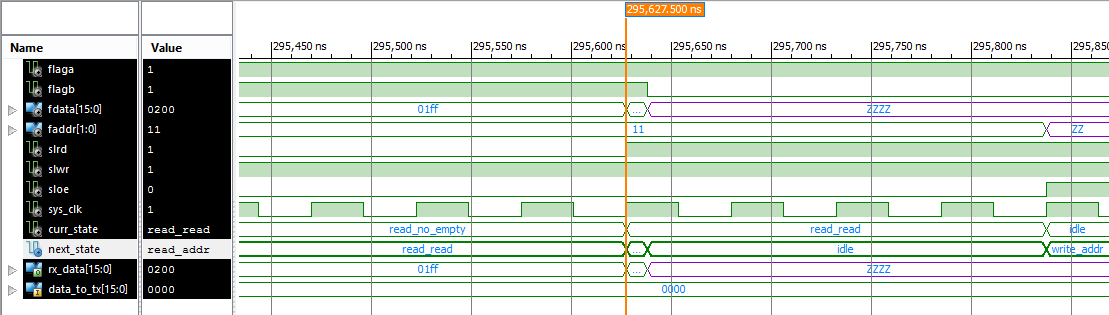
\includegraphics[width=\textwidth]{tb_if_rd_end}
%		}
%\end{frame}
%\begin{frame}{Test bench - Escritura en la interfaz}
%	\only<1>{
%		\centering
%		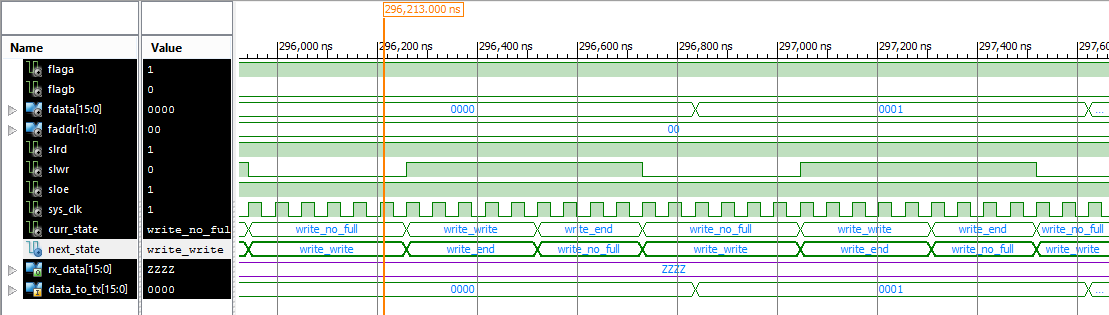
\includegraphics[width=\textwidth]{tb_if_wr_mef}\\
%		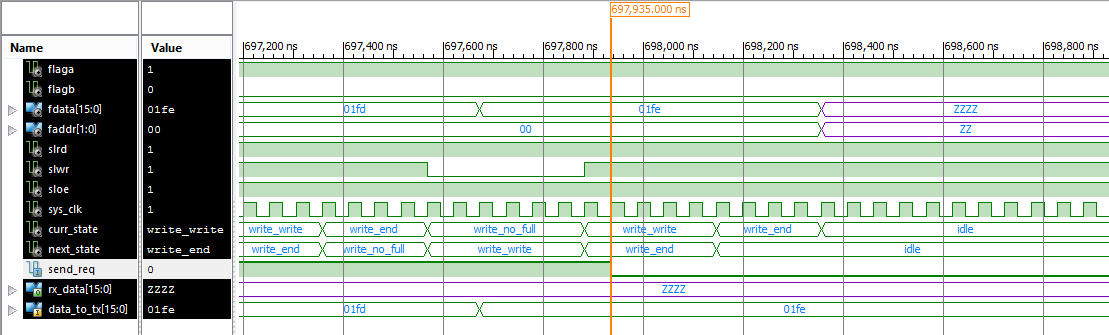
\includegraphics[width=\textwidth]{tb_if_wr_end}}
%	\only<2>{
%		\centering
%		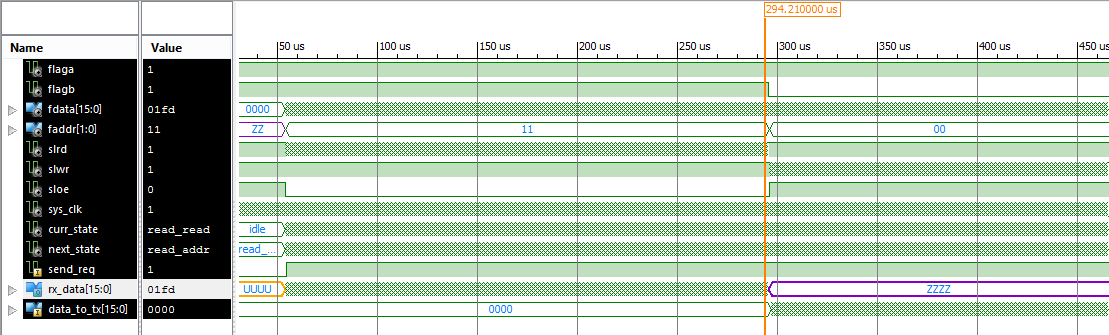
\includegraphics[width=\textwidth]{tb_if_snd}\\
%		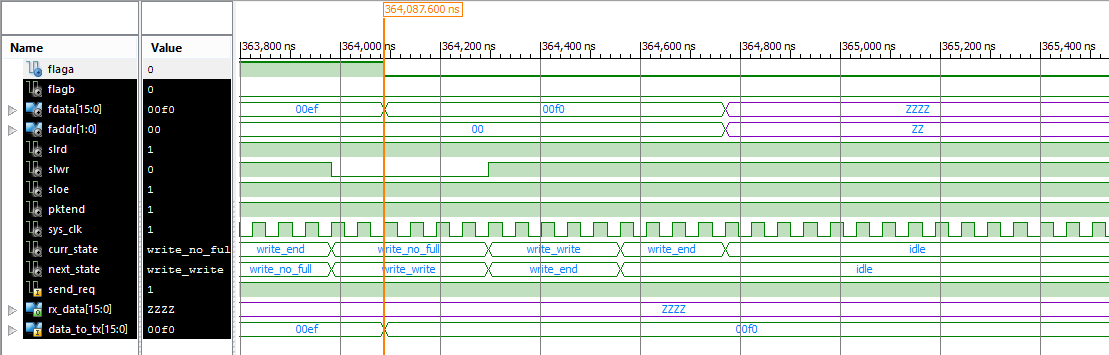
\includegraphics[width=\textwidth]{tb_if_fflag_end}}
%\end{frame}
